\section{Results and Analysis}

\subsection{Overview of Results}

This section presents the measured results for all three access control scenarios across the three evaluation metrics: cost per access attempt (M1), average CPU utilization (M2), and average memory utilization (M3). All scenarios were executed with 20 bookings and 20 corresponding access attempts under identical infrastructure conditions.

Table~\ref{tab:results_overview} provides a summary of all measured values. Cost figures include the fixed monthly infrastructure baseline of \$4.43 amortized over 1{,}000 access attempts, making the comparison practically meaningful.

\begin{table}[H]
\centering
\caption{Measured results per scenario (cost at 1{,}000 monthly access attempts)}
\label{tab:results_overview}
\begin{tabular}{p{1.5cm}p{2.2cm}p{3.2cm}p{2.6cm}p{2.6cm}}
\hline
\textbf{Case} & \textbf{Security Level} & \textbf{M1 (Total/Month)} & \textbf{M2 (Avg. CPU)} & \textbf{M3 (Avg. Mem.)} \\
\hline
Case 1 & Low    & \$4.43 & 3.1\% & 41.2\% \\
Case 2 & Medium & \$5.43 & 3.4\% & 41.8\% \\
Case 3 & High   & \$5.53 & 3.3\% & 42.1\% \\
\hline
\end{tabular}
\end{table}

\subsection{Cost per Access Attempt (M1)}

The total monthly cost of operating the system consists of two components: a fixed infrastructure baseline that is invariant across all scenarios, and a variable per-attempt cost that depends on the managed AWS services invoked during each access event.

\paragraph{Fixed Infrastructure Baseline.}
The shared ECS Fargate task, RDS \texttt{db.t3.micro} instance, VPC, and ALB components incur a combined fixed cost of \$4.43 per month regardless of which access control scenario is active or how many access attempts are processed. This baseline represents the minimum operational cost of running the system and is identical for all three cases.

\paragraph{Variable Cost per Attempt.}
Case 1 invokes no external AWS services at access time and therefore adds no variable cost on top of the baseline. Case 2 introduces a single call to Amazon Rekognition \texttt{SearchFacesByImage} per access attempt, priced at \$0.001 per image (AWS pricing, June 2026). Case 3 is identical to Case 2 but additionally dispatches the Nuki code via Amazon SES, priced at \$0.0001 per message, bringing its per-attempt variable cost to \$0.0011.

Table~\ref{tab:cost_breakdown} breaks down the variable cost components per scenario.

\begin{table}[H]
\centering
\caption{Variable cost breakdown per access attempt (AWS pricing, June 2026)}
\label{tab:cost_breakdown}
\begin{tabular}{p{1.5cm}p{3.5cm}p{2.8cm}p{2.8cm}}
\hline
\textbf{Case} & \textbf{Service Invocation} & \textbf{Unit Price (USD)} & \textbf{Variable Total} \\
\hline
Case 1 & None & -- & \$0.0000 \\
\hline
Case 2 & Rekognition \texttt{SearchFacesByImage} & \$0.0010 & \$0.0010 \\
\hline
\multirow{2}{*}{Case 3} & Rekognition \texttt{SearchFacesByImage} & \$0.0010 & \multirow{2}{*}{\$0.0011} \\
                         & Amazon SES (1 message)                  & \$0.0001 & \\
\hline
\end{tabular}
\end{table}

\paragraph{Total Monthly Cost.}
Table~\ref{tab:monthly_cost} combines the fixed baseline with the projected variable cost at three usage volumes to illustrate how the cost structure shifts with scale.

\begin{table}[H]
\centering
\caption{Total projected monthly cost including fixed infrastructure baseline}
\label{tab:monthly_cost}
\begin{tabular}{p{1.5cm}p{2.0cm}p{2.2cm}p{2.2cm}p{2.2cm}}
\hline
\textbf{Case} & \textbf{Fixed} & \textbf{100 att.} & \textbf{1{,}000 att.} & \textbf{10{,}000 att.} \\
\hline
Case 1 & \$4.43 & \$4.43 & \$4.43  & \$4.43  \\
Case 2 & \$4.43 & \$4.53 & \$5.43  & \$14.43 \\
Case 3 & \$4.43 & \$4.54 & \$5.53  & \$15.43 \\
\hline
\end{tabular}
\end{table}

At low usage (100 attempts/month), the fixed baseline dominates and all three scenarios cost nearly the same (\$4.43 to \$4.54). At 1{,}000 attempts the security surcharge of Case 3 over Case 1 is \$1.10 (+24.8\%). At 10{,}000 attempts the variable cost of Case 3 (\$11.00) exceeds the fixed infrastructure cost by a factor of approximately 2.5, making the choice of security scenario the primary cost driver.

\subsection{CPU and Memory Utilization (M2, M3)}

Both CPU and memory utilization of the Access Service remained at comparable levels across all three scenarios, as shown in Table~\ref{tab:results_overview}. The observed variation (3.1\% to 3.4\% for CPU, 41.2\% to 42.1\% for memory) falls within the margin of measurement noise inherent to one-minute CloudWatch sampling and does not represent a meaningful operational difference.

This outcome is consistent with the architectural design of the system. The Access Service is I/O-bound: its main role at access time is to invoke external managed services (Rekognition, SES) and await their responses. The computationally intensive operations, namely face recognition inference and email relay, are executed on AWS-managed infrastructure and do not contribute to the Access Service's CPU or memory footprint. The additional Rekognition and SES calls introduced by Cases 2 and 3 manifest as network round-trips and API latency, not as additional local compute load.

The memory footprint of approximately 41 to 42\% across all scenarios corresponds to the baseline JVM heap usage of the Spring Boot application and the in-memory image buffer used during face verification. Since the selfie image is passed directly to the Rekognition API and not persisted, its transient allocation does not accumulate over repeated attempts.

Consequently, M2 and M3 are not suitable discriminating metrics for the scenarios evaluated in this work. The relevant resource impact of higher security levels is captured entirely by M1.

\subsection{Comparison of Security Levels}

Figure~\ref{fig:cost_comparison} illustrates the total monthly cost at 1{,}000 access attempts across the three scenarios, combining the fixed baseline with scenario-specific variable costs. The step from Case 1 to Case 2 represents the dominant cost increment, driven entirely by the Rekognition integration. The additional surcharge from Case 2 to Case 3 (SES delivery) is marginal in comparison.

\begin{figure}[H]
\centering
\resizebox{0.78\linewidth}{!}{%
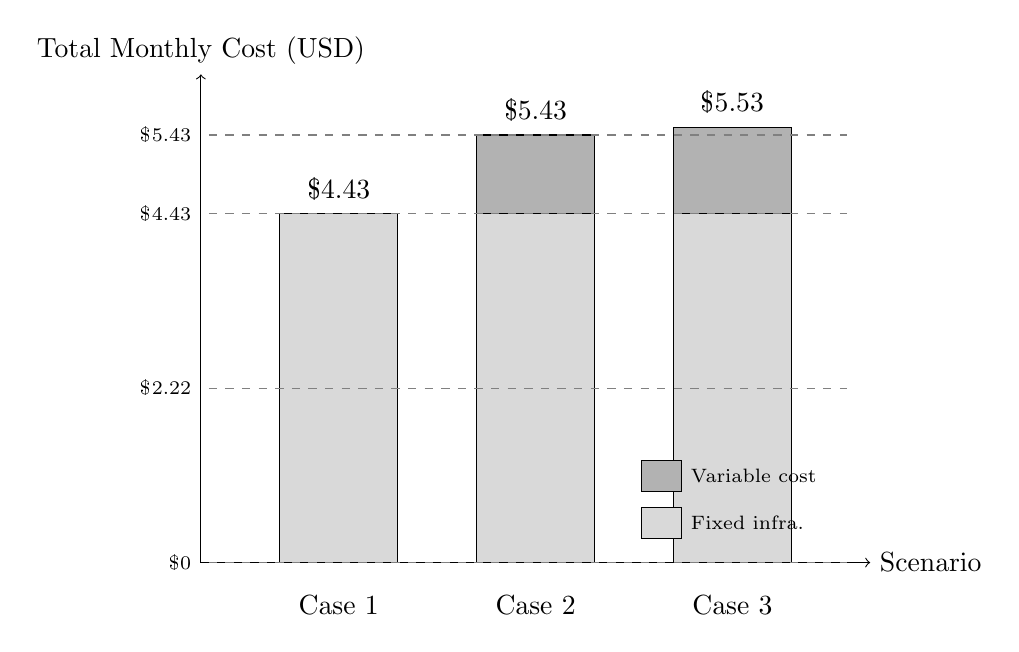
\begin{tikzpicture}
    \draw[->] (0,0) -- (8.5,0) node[right] {Scenario};
    \draw[->] (0,0) -- (0,6.2) node[above] {Total Monthly Cost (USD)};

    % Fixed baseline layer (gray)
    \draw[fill=gray!30] (1,0)   rectangle (2.5,4.43);
    \draw[fill=gray!30] (3.5,0) rectangle (5.0,4.43);
    \draw[fill=gray!30] (6.0,0) rectangle (7.5,4.43);

    % Variable cost layer (darker)
    \draw[fill=gray!60] (3.5,4.43) rectangle (5.0,5.43);
    \draw[fill=gray!60] (6.0,4.43) rectangle (7.5,5.53);

    \node[below] at (1.75,-0.3) {Case 1};
    \node[below] at (4.25,-0.3) {Case 2};
    \node[below] at (6.75,-0.3) {Case 3};

    \node[above] at (1.75,4.48) {\$4.43};
    \node[above] at (4.25,5.48) {\$5.43};
    \node[above] at (6.75,5.58) {\$5.53};

    \foreach \y/\label in {0/\$0, 2.215/\$2.22, 4.43/\$4.43, 5.43/\$5.43} {
        \draw[gray, dashed] (0.1,\y) -- (8.2,\y);
        \node[left, font=\scriptsize] at (0,\y) {\label};
    }

    % Legend
    \draw[fill=gray!30] (5.6,0.3) rectangle (6.1,0.7);
    \node[right, font=\scriptsize] at (6.1,0.5) {Fixed infra.};
    \draw[fill=gray!60] (5.6,0.9) rectangle (6.1,1.3);
    \node[right, font=\scriptsize] at (6.1,1.1) {Variable cost};
\end{tikzpicture}%
}
\caption{Total monthly cost by scenario at 1{,}000 access attempts (fixed + variable).}
\label{fig:cost_comparison}
\end{figure}

\subsection{Interpretation of Findings}

The results confirm that the fixed infrastructure baseline (\$4.43/month) is the dominant cost component at low to moderate access volumes. At 1{,}000 monthly attempts, it accounts for 80\% of the total cost in Case 3. The choice of security scenario therefore has limited practical cost impact until access volumes reach several thousand attempts per month.

When variable costs become significant at higher volumes, the primary driver is the integration of Amazon Rekognition for biometric face verification (Case 2 and 3), not the out-of-band delivery channel (Case 3 only). Rekognition accounts for \$0.001 of the \$0.0011 per-attempt cost in Case 3, approximately 91\% of the total variable cost of the highest-security scenario. The SES surcharge of \$0.0001 per attempt is negligible by comparison.

The absence of measurable differences in CPU and memory utilization across scenarios reflects the delegation model inherent to cloud-native architectures: managed services externalize computational work, making on-task resource metrics an unreliable proxy for security-related operational cost. The true cost of higher security assurance is best captured through API billing metrics rather than infrastructure utilization metrics.
